%%%%%%%%%%%%%%%%%%%%%%%%%%%%%%%%%%%%%%%%%%%%%%%%%%%%%%%%%%%%%%%%%%%%%%%%%%%%
% Implementation
%%%%%%%%%%%%%%%%%%%%%%%%%%%%%%%%%%%%%%%%%%%%%%%%%%%%%%%%%%%%%%%%%%%%%%%%%%%%

\chapter{Implementation}
\label{chapter:Implementation}
%In this chapter, you should discuss the different stages you followed to have a successful implementation for your final product.\\
%\newline
%\textbf{It is highly encouraged to utilize diagrams and illustrations.} 


%% ============================================================
%% Chapter 6 – Implementation
%% Add to preamble: \usepackage{listings}  \usepackage{xcolor}
%% ============================================================

\definecolor{codegray}{rgb}{0.95,0.95,0.95}
\definecolor{keywordcolor}{rgb}{0.13,0.13,0.60}

This chapter describes the end-to-end implementation of \textit{SoleMate}, the system comprises three tightly coupled layers: an Arduino Nano~33~BLE
embedded device that acquires and encrypts sensor data; an Android application that decrypts,
processes, and visualises that data; and a lightweight Node.js back-end that relays automated
health reports by email.  Each section below details one major subsystem, cross-referencing
specific source files and data structures throughout.


\section{System Architecture Overview}
\label{sec:arch}

Figure~\ref{fig:arch_overview} provides a high-level view of the complete system architecture.
Sensor data originates on the wearable device and travels over a Bluetooth Low Energy (BLE)
channel to the mobile application, where it is decrypted, analysed by a machine-learning model,
and rendered in real time.  Periodic automated reports are forwarded to a cloud email relay.

\begin{figure}[htbp]
  \centering
  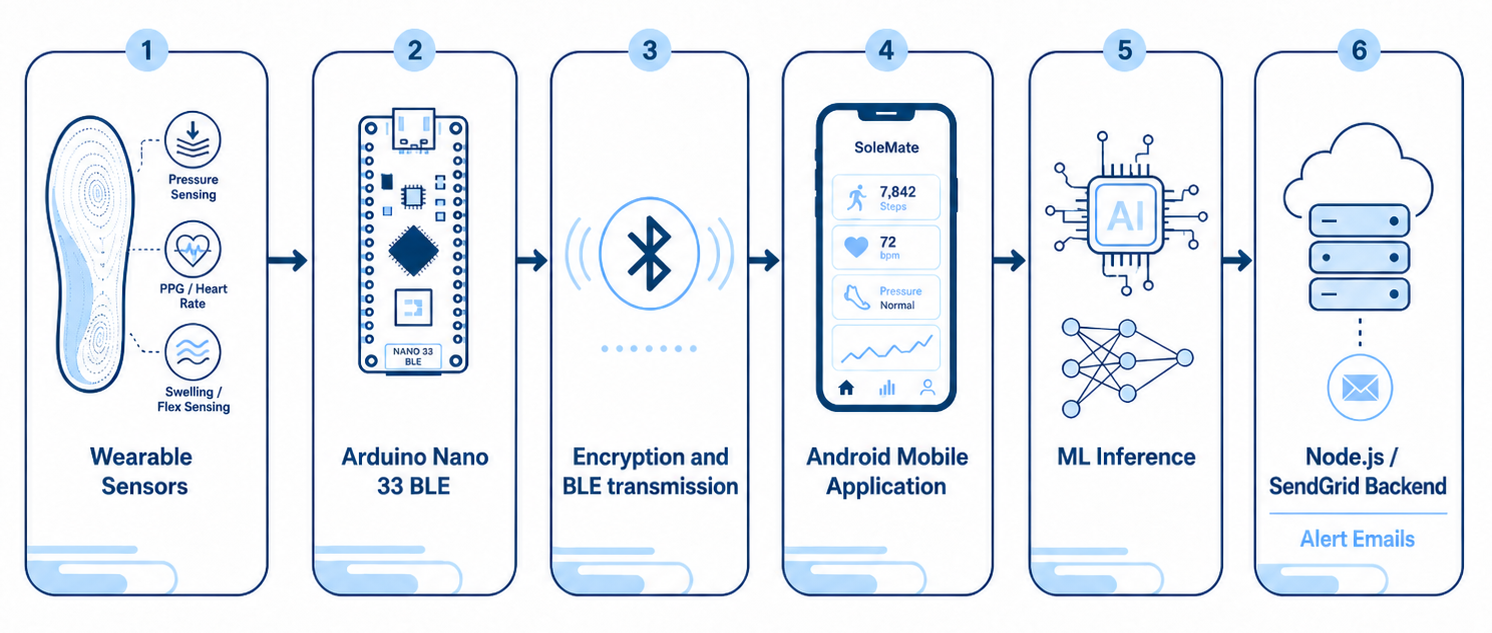
\includegraphics[width=0.95\textwidth]{FYP_Template_Spring/Figures/system_architecture.png}
  \caption{High-level architecture of the SoleMate system.}
  \label{fig:arch_overview}
\end{figure}

The full data pipeline can be summarized in four stages.

\begin{enumerate}[label=\textbf{Stage~\arabic*.}, leftmargin=*, itemsep=4pt]
  \item \textbf{Acquisition.}  Four sensor modules (IMU, PPG, flex, and pressure matrix) sample
        physiological signals on the Arduino firmware at rates between 5\,Hz and 100\,Hz.
  \item \textbf{Encryption and transmission.}  Each data type is independently encrypted with
        AES-128-CBC using a key derived from a session-specific ECDH shared secret, then
        broadcast over BLE via dedicated GATT characteristics.
  \item \textbf{Reception and decryption.}  The Android application discovers the device,
        completes the key exchange, and continuously decrypts incoming notifications.
  \item \textbf{Processing and presentation.}  Decrypted values feed real-time charts, a
        plantar-pressure heatmap, a CapsNet-based ataxia classifier, a machine-learning
        blood-pressure estimator, and an automated email-sharing worker.
\end{enumerate}

Table~\ref{tab:tech_stack} summarises the principal technologies used across all layers.

\begin{table}[htbp]
  \centering
  \caption{Technology stack summary.}
  \label{tab:tech_stack}
  \begin{tabularx}{\textwidth}{l l X}
    \hline
    \textbf{Layer} & \textbf{Technology} & \textbf{Role} \\
    \hline
    Firmware        & Arduino C++ / ArduinoBLE       & Sensor acquisition, encryption, BLE advertising \\
    Communication  & Bluetooth Low Energy (GATT)    & Wireless data transfer \\
    Cryptography   & ECDH (secp256r1) + AES-128-CBC & Session key exchange and prototype data encryption \\
    Mobile UI      & Kotlin / Material Design       & Visualisation, settings, authentication \\
    ML training    & Python / PyTorch               & CapsNet-based ataxia classifier training \\
    ML inference   & PyTorch ExecuTorch 1.2.0       & On-device blood pressure estimation \\
    Signal proc.   & JTransforms (JVM FFT)          & STFT spectrogram computation \\
    Email relay    & Node.js + SendGrid             & Automated health-report delivery \\
    \hline
  \end{tabularx}
\end{table}

% ------------------------------------------------------------
\section{Hardware Platform}
\label{sec:hardware}
% ------------------------------------------------------------



\subsection{Arduino Nano 33 BLE}
\label{subsec:hw_arduino}

The wearable device is built around the \textbf{Arduino Nano~33~BLE}, a compact
($45 \times 18$\,mm) microcontroller module based on the Nordic nRF52840 SoC.  The nRF52840
integrates an ARM Cortex-M4F processor (64\,MHz), 1\,MB Flash, 256\,KB SRAM, and a dedicated
BLE 5.0 radio — making it well-suited for a battery-powered wearable that must handle
encryption, sensor polling, and wireless transmission concurrently.  The board also provides
14 digital I/O pins, 8 analogue inputs with 12-bit resolution, and I\textsuperscript{2}C/SPI
buses required to interface the sensor suite.

\begin{figure}[H]
  \centering
  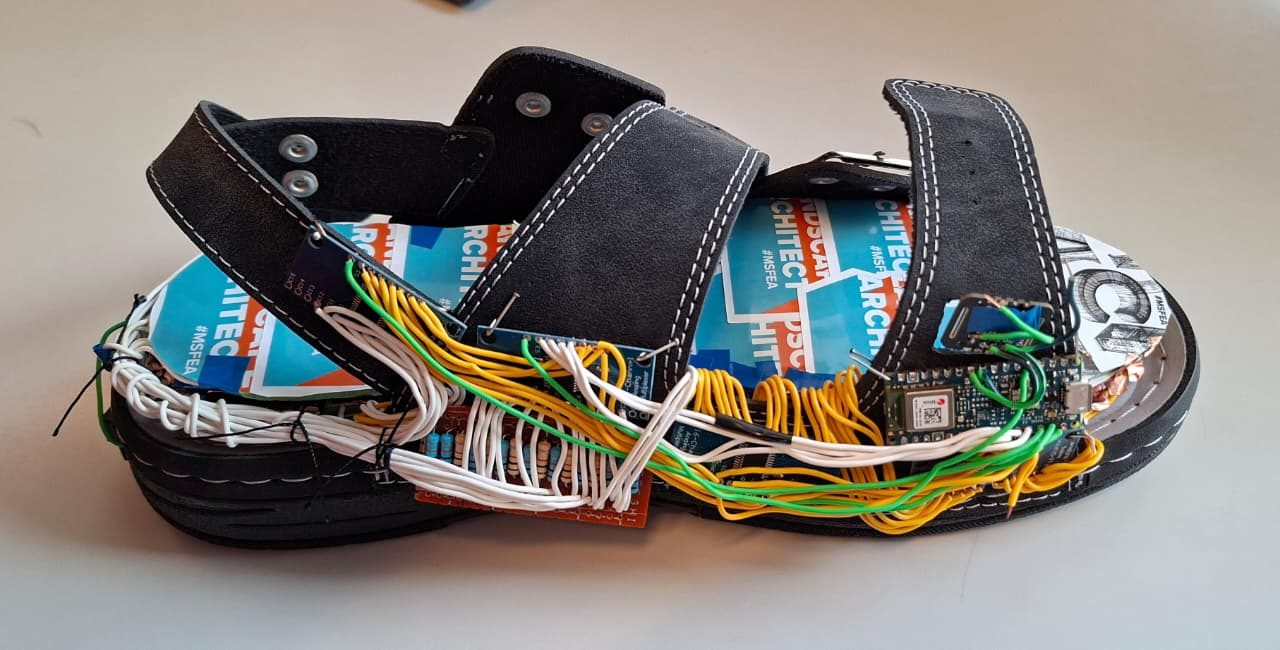
\includegraphics[width=0.95\textwidth]{FYP_Template_Spring/Figures/hardware.jpeg}
  \caption{The SoleMate wearable hardware: Arduino Nano~33~BLE with attached sensors.}
  \label{fig:hw_board}
\end{figure}

\subsection{Sensor Suite}
\label{subsec:hw_sensors}

Four distinct sensing modalities were integrated to cover the clinical parameters of interest.
Table~\ref{tab:sensors} provides a concise specification of each.

\begin{table}[htbp]
  \centering
  \caption{Sensor specifications on the SoleMate wearable device.}
  \label{tab:sensors}
  \begin{tabularx}{\textwidth}{l l l X}
    \hline
    \textbf{Sensor} & \textbf{Model} & \textbf{Interface} & \textbf{Purpose / Key Parameters} \\
    \hline
    IMU           & BMI270\_BMM150  & I\textsuperscript{2}C & 6-axis inertial; $\pm2$g accel, $\pm250$\,dps gyro @ 10\,Hz; gait analysis \\
    PPG           & MAX30102        & I\textsuperscript{2}C & IR + Red LED photoplethysmography; 100\,Hz; heart rate (45–180\,BPM), SpO\textsubscript{2} \\
    Flex (×4)     & Analogue bend   & ADC (A0, A1)   & Ankle flexion; 5\,Hz; edema classification via deviation from calibrated baseline \\
    Pressure matrix & Custom 16$\times$48 & MUX + ADC & 768-cell plantar-foot map; 12-bit ADC per cell; foot-pressure distribution \\
    \hline
  \end{tabularx}
\end{table}

\begin{figure}[H]
   \centering
   \includegraphics[width=0.95\textwidth]{FYP_Template_Spring/Figures/sensor_placement.png}
  \caption{Sensor placement on the SoleMate wearable assembly.}
  \label{fig:hw_placement}
\end{figure}

% ------------------------------------------------------------
\section{Arduino Firmware}
\label{sec:firmware}
% ------------------------------------------------------------

\subsection{Firmware Structure and Initialisation}
\label{subsec:fw_structure}

\noindent The firmware (\texttt{arduinobackend.ino}) follows a modular design: each sensor type is
encapsulated in its own \texttt{.cpp}/\texttt{.h} module (\texttt{imu\_reader},
\texttt{ppg\_reader}, \texttt{flex\_reader}, \texttt{pressure\_reader},
\texttt{ppg\_waveform\_collect}), with cross-cutting concerns such as encryption and key exchange
handled by dedicated \texttt{encryption} and \texttt{key\_exchange} modules.  The main sketch
registers BLE services, wires interrupt-style callbacks, and runs a cooperative polling loop. \\


\noindent Serial logging is gated by a \texttt{serial\_log} abstraction so that debug output can be disabled at compile time without altering the main logic.  Sensor modules are conditionally compiled using pre-processor flags (\texttt{SENSOR\_IMU\_ENABLED}, \texttt{SENSOR\_PPG\_ENABLED},
etc.), which allows the same firmware to be built for hardware configurations that omit one or
more sensors. \\


\noindent Algorithm~\ref{alg:fw_init} summarises the initialisation sequence executed in \texttt{setup()}.

\begin{algorithm}[htbp]
\caption{Arduino Firmware Initialisation (\texttt{setup()})}
\label{alg:fw_init}
\begin{algorithmic}[1]
  \STATE Initialise serial port at 2\,000\,000\,bps (non-blocking, debug only)
  \STATE Set analogue resolution to 12 bits
  \STATE Initialise IMU (BMI270), PPG (MAX30102), flex sensors, pressure matrix
  \STATE Generate ephemeral ECDH key pair (secp256r1)
  \STATE Register BLE Key Exchange Service (\texttt{9a8b1001-\ldots}) with write/read callbacks
  \STATE Register BLE Wearable Service (\texttt{9a8b0001-\ldots}) with 8 characteristics
  \STATE Attach \texttt{onPhoneKeyWritten()} callback to the Phone Public Key characteristic
  \STATE Start BLE advertising as \textquotedblleft SoleMate\textquotedblright
\end{algorithmic}
\end{algorithm}

\subsection{IMU Sensor Module — Gait Analysis}
\label{subsec:fw_imu}

\noindent The \texttt{imu\_reader} module interfaces the on-board BMI270 inertial measurement unit over
I\textsuperscript{2}C.  Each read returns a \texttt{IMUData} struct containing six
floating-point fields: three axes of linear acceleration ($a_x, a_y, a_z$) in units of $g$, and
three axes of angular velocity ($\omega_x, \omega_y, \omega_z$) in degrees per second.
The sensor is configured with a $\pm2$g acceleration range and $\pm250$\,dps gyroscope range,
sampled at 10\,Hz to match the BLE notification cadence.  These values are transmitted as a
comma-separated string of the form \texttt{"ax,ay,az"} for the accelerometer characteristic and
\texttt{"gx,gy,gz"} for the gyroscope characteristic, each encrypted before transmission. \\



\subsection{PPG Sensor Module — Heart Rate and SpO\textsubscript{2}}
\label{subsec:fw_ppg}

\noindent The MAX30102 pulse-oximetry sensor is operated in two-LED (IR + Red) photoplethysmography mode.
The \texttt{ppg\_reader} module implements a peak-detection algorithm over the IR channel to
derive instantaneous heart rate, clamped to the physiologically plausible range of 45–180\,BPM.
Blood-oxygen saturation (SpO\textsubscript{2}) is computed from the ratio $R$ of AC-to-DC
amplitudes of the Red and IR channels using the empirical relation:

\begin{equation}
  \mathrm{SpO_2} = (0.0092R + 0.963) \times 100\%
  \label{eq:spo2}
\end{equation}

\noindent A minimum IR threshold of 20\,000 ADC counts is used for finger-presence detection; readings
below this threshold are discarded.  Heart rate and SpO\textsubscript{2} values are formatted as
short ASCII strings (\texttt{"72"} and \texttt{"98.5"} respectively), padded, encrypted, and
written to their respective BLE characteristics at 100\,Hz.

\subsection{Flex Sensor Module — Swelling Detection}
\label{subsec:fw_flex}
\noindent The swelling-detection subsystem was implemented using four flex sensors arranged around the ankle in a dual-level circumferential configuration. Unlike the earlier two-sensor version, %i believe we should mention this before as a design iteration
which only estimated swelling from a combined deviation value, the final implementation uses two sensors at an upper ankle level and two sensors at a lower ankle level. This arrangement allows the system to estimate two local ankle circumferences and then estimate a localized ankle-segment volume. The purpose of this design is to provide a more physically meaningful swelling indicator, since swelling is better represented as a change in local volume rather than as a simple raw sensor deviation. \\


\noindent Each flex sensor is connected to the microcontroller through an independent voltage-divider circuit. One terminal of the flex sensor is connected to the 3.3~V supply supplied from the arduino, while the other terminal is connected to an analogue input pin and to a fixed 47 kilo ohm resistor connected to ground. As the ankle curves or swells, the flex sensor bends varying its resistance and consequently producing a corresponding change in the analogue voltage measured by the microcontroller ADC. The four sensors are assigned to the firmware according to their physical placement: upper-left (UL), upper-right (UR), lower-left (LL), and lower-right (LR). In the implemented prototype, the corrected analogue pin mapping was UL~=~A6, UR~=~A3, LL~=~A2, and LR~=~A1. \\


\noindent Since flex sensors measure bending rather than circumference directly, a calibration stage was required to map each raw ADC reading to an estimated circumference in centimeters. During calibration, the ankle circumference was manually measured using a flexible measuring tape at both the upper and lower sensor levels. At each known circumference, the corresponding raw ADC readings from all four flex sensors were recorded. Sensor-specific calibration curves were then generated using a linear estimated fit of the form

\begin{equation}
    C_i = m_i R_i + b_i,
    \label{eq:flex_calibration}
\end{equation}

\noindent where $C_i$ is the estimated circumference from sensor $i$, $R_i$ is the filtered raw ADC reading, and $m_i$ and $b_i$ are the slope and intercept obtained experimentally from the calibration curve of that sensor. Separate calibration equations were used for the four sensors because each flex sensor had a slightly different bending response due to placement, soldering, contact pressure, and curvature. The upper sensors were calibrated against the measured upper ankle circumference, while the lower sensors were calibrated against the measured lower ankle circumference. \\


\noindent To reduce noise, the firmware first computes an averaged raw value for each sensor by taking multiple ADC samples. The calibrated circumference estimates are then computed as

\begin{equation}
    C_{UL} = m_{UL}R_{UL} + b_{UL},
\end{equation}

\begin{equation}
    C_{UR} = m_{UR}R_{UR} + b_{UR},
\end{equation}

\begin{equation}
    C_{LL} = m_{LL}R_{LL} + b_{LL},
\end{equation}

\begin{equation}
    C_{LR} = m_{LR}R_{LR} + b_{LR}.
\end{equation}

\noindent The upper and lower ankle circumferences are then estimated by averaging the corresponding pair of sensors:

\begin{equation}
    C_1 = \frac{C_{UL} + C_{UR}}{2},
    \label{eq:upper_circ}
\end{equation}

\begin{equation}
    C_2 = \frac{C_{LL} + C_{LR}}{2},
    \label{eq:lower_circ}
\end{equation}

\noindent where $C_1$ represents the estimated upper circumference and $C_2$ represents the estimated lower circumference. These two circumferences are used to estimate the volume of the monitored ankle region. In the firmware, this region is modeled as a truncated cone, since the upper and lower circumference levels may not be equal. The circumferences are first converted to radii using

\begin{equation}
    r_1 = \frac{C_1}{2\pi},
    \qquad
    r_2 = \frac{C_2}{2\pi},
\end{equation}

\noindent and the localized ankle-segment volume is computed as

\begin{equation}
    V_{\text{ankle}} =
    \frac{\pi D}{3}
    \left(
    r_1^2 + r_1 r_2 + r_2^2
    \right),
    \label{eq:frustum_volume}
\end{equation}

\noindent where $D$ is the vertical distance between the upper and lower sensor levels. This frustum-based formulation was selected because it accounts for the two different circumference levels independently, making it more representative of the actual ankle segment geometry than a simple cylindrical approximation using only an averaged circumference. \\

\noindent A personalized baseline volume is established when the device is worn in the normal, non-swollen condition. The firmware computes a stable baseline by repeatedly estimating the ankle volume and averaging multiple readings to reduce random fluctuations. During real-time operation, the current ankle volume is compared to the stored baseline volume, and the swelling deviation is calculated as

\begin{equation}
    \Delta V(\%) =
    \frac{V_{\text{current}} - V_{\text{baseline}}}
    {V_{\text{baseline}}}
    \times 100.
    \label{eq:volume_deviation}
\end{equation}

\noindent The resulting percentage deviation is mapped to four swelling severity classes, as shown in Table~\ref{tab:edema}. The classification thresholds were implemented as percentage changes from the user-specific baseline, making the subsystem adaptive to individual ankle size rather than relying on fixed raw ADC thresholds.

\begin{table}[htbp]
  \centering
  \caption{Swelling classification thresholds based on localized ankle-volume deviation from baseline.}
  \label{tab:edema}
  \begin{tabularx}{\textwidth}{l l X}
    \hline
    \textbf{Label} & \textbf{Volume Deviation} & \textbf{Interpretation} \\
    \hline
    \texttt{none}     & $<5\%$        & No significant swelling relative to baseline \\
    \texttt{mild}     & $5$--$10\%$   & Mild swelling / early measurable increase \\
    \texttt{moderate} & $>10$--$30\%$ & Moderate swelling requiring monitoring \\
    \texttt{severe}   & $>30\%$       & Severe swelling requiring prompt attention \\
    \hline
  \end{tabularx}
\end{table}

\noindent To improve real-time stability, the firmware does not classify swelling from a single instantaneous reading. Instead, it estimates a stable volume by repeating the volume calculation several times and averaging the resulting values. During this process, the firmware also computes the spread between the minimum and maximum volume estimates to detect unstable sensor contact or strap movement. If the spread exceeds a predefined tolerance, a warning is generated, indicating that the reading may be affected by sensor repositioning or inconsistent contact. In addition, hysteresis is applied around the severe-swelling boundary to reduce fluctuations between the moderate and severe labels when the percentage deviation is close to the $30\%$ threshold. \\

%\noindent The final output of the flex-sensor module therefore includes the calibrated upper circumference, calibrated lower circumference, localized ankle-segment volume, percentage volume deviation from baseline, and the corresponding swelling severity label. This implementation provides a more interpretable swelling-detection pipeline than the previous raw-deviation approach, because each stage of the process corresponds to a physical quantity: sensor bending, circumference, local volume, and percentage change from the user's baseline. \\

\subsection{Pressure Matrix Module — Plantar Foot Mapping}
\label{subsec:fw_pressure}

\noindent The plantar-pressure sensor is a custom resistive matrix of $16 \times 48 = 768$ cells arranged in row-major order to cover the entire plantar surface of a shoe insole.  Rows are selected via a 4:16 analogue multiplexer (control pins 6–9); each of the three column banks (48 columns)
is driven by a secondary multiplexer (control pins 2–5) and read through three signal lines
(pins 10–12) plus an additional row-signal on A2.  A settle time of 2\,µs is applied between
MUX selection and ADC sampling to allow the signal to stabilize. \\

\noindent The 12-bit ADC values (0–4095) are packed into compact BLE packets using the structure in
Table~\ref{tab:pressure_packet}.  Each packet carries eight 12-bit samples (96 bits) encoded into
12 bytes, preceded by an 8-byte header containing magic bytes \texttt{0xA5~0x5A}, the frame
sequence number, the packet index within the frame, and a row identifier.  A full frame of 768
cells requires 96 such packets. \\

\begin{table}[htbp]
  \centering
  \caption{Pressure matrix BLE packet structure (24 bytes total after encryption).}
  \label{tab:pressure_packet}
  \begin{tabularx}{\textwidth}{l l l X}
    \hline
    \textbf{Byte(s)} & \textbf{Field} & \textbf{Size} & \textbf{Description} \\
    \hline
    0–1   & Magic         & 2\,B  & \texttt{0xA5 0x5A} — frame synchronisation \\
    2     & Frame seq.    & 1\,B  & Rolling frame sequence counter \\
    3     & Packet index  & 1\,B  & Packet number within the current frame (0–95) \\
    4     & Row ID        & 1\,B  & Row index (0–15) \\
    5–7   & Reserved      & 3\,B  & Future use / padding \\
    8–19  & Ciphertext    & 12\,B & AES-128-CBC of 12-byte 12-bit sample payload \\
    \hline
  \end{tabularx}
\end{table}

\noindent Scanning is implemented as a \textit{non-blocking} state machine (\texttt{pressure\_scan\_step})
that processes a configurable number of columns per call, yielding control between IMU reads so
that no sensor type starves.  Once all 96 packets of a frame are assembled, the \texttt{PressureFrame} struct is made available for BLE notification. \\


\section{Bluetooth Low Energy Communication Protocol}
\label{sec:ble}


\subsection{GATT Service Architecture}
\label{subsec:ble_gatt}

The firmware exposes two GATT services.  The \textit{Key Exchange Service} (UUID prefix
\texttt{9a8b1001-\ldots}) provides the secure channel for public-key distribution and is only
active during the handshake phase.  The primary \textit{Wearable Service} is identified by
\texttt{9a8b0001-6d5e-4c10-b6d9-1f25c09d9e00} and hosts the streaming sensor characteristics
\texttt{9a8b0002-\ldots} through \texttt{9a8b0008-\ldots}.
Table~\ref{tab:ble_chars} enumerates these seven characteristics (the Android client registers
notifications for each discovered characteristic under this service).

\begin{table}[htbp]
  \centering
  \caption{BLE GATT characteristics exposed by the wearable service.}
  \label{tab:ble_chars}
  \begin{tabularx}{\textwidth}{l l l X}
    \hline
    \textbf{UUID (suffix)} & \textbf{Properties} & \textbf{Size} & \textbf{Data type} \\
    \hline
    \texttt{9a8b0002-\ldots} & Read, Notify & 81\,B & Step count (IMU-derived; encrypted ASCII integer) \\
    \texttt{9a8b0003-\ldots} & Read, Notify & 81\,B & Motion state (IMU-derived; encrypted label) \\
    \texttt{9a8b0004-\ldots} & Read, Notify & 81\,B & Heart rate (BPM as ASCII) \\
    \texttt{9a8b0005-\ldots} & Read, Notify & 81\,B & SpO\textsubscript{2} (\% as ASCII) \\
    \texttt{9a8b0006-\ldots} & Read, Notify & 81\,B & edema (\texttt{label,dev,dev1,dev2}) \\
    \texttt{9a8b0007-\ldots} & Read, Notify & 24\,B & Pressure matrix packets \\
    \texttt{9a8b0008-\ldots} & Read, Notify & 81\,B & PPG waveform chunk (raw ADC samples) \\
    \hline
    \multicolumn{4}{l}{\textit{Key Exchange Service}} \\
    \hline
    \texttt{9a8b1002-\ldots} & Write        & 65\,B & Phone public key (uncompressed EC point) \\
    \texttt{9a8b1003-\ldots} & Read         & 65\,B & Peripheral public key (uncompressed EC point) \\
    \hline
  \end{tabularx}
\end{table}

\noindent For all sensor characteristics except pressure, the 81-byte payload format is:
\texttt{[1 byte: ciphertext length][up to 80 bytes: AES-128-CBC ciphertext]}.
On Android, ATT MTU negotiation is deferred until \emph{after} all notification descriptors (CCCD
writes) have been queued for the wearable characteristics: the client then requests
\texttt{requestMtu(247)} to maximise the negotiated ATT payload on modern stacks (the effective
value is still subject to phone/peripheral limits).  This ordering avoids a known class of Android
GATT bugs where requesting MTU too early during service discovery can stall discovery.

\subsection{Connection and Notification Sequence}
\label{subsec:ble_sequence}

Figure~\ref{fig:ble_seq} illustrates the connection and key-exchange sequence between the Android
application and the firmware.

\begin{figure}[H]
   \centering
   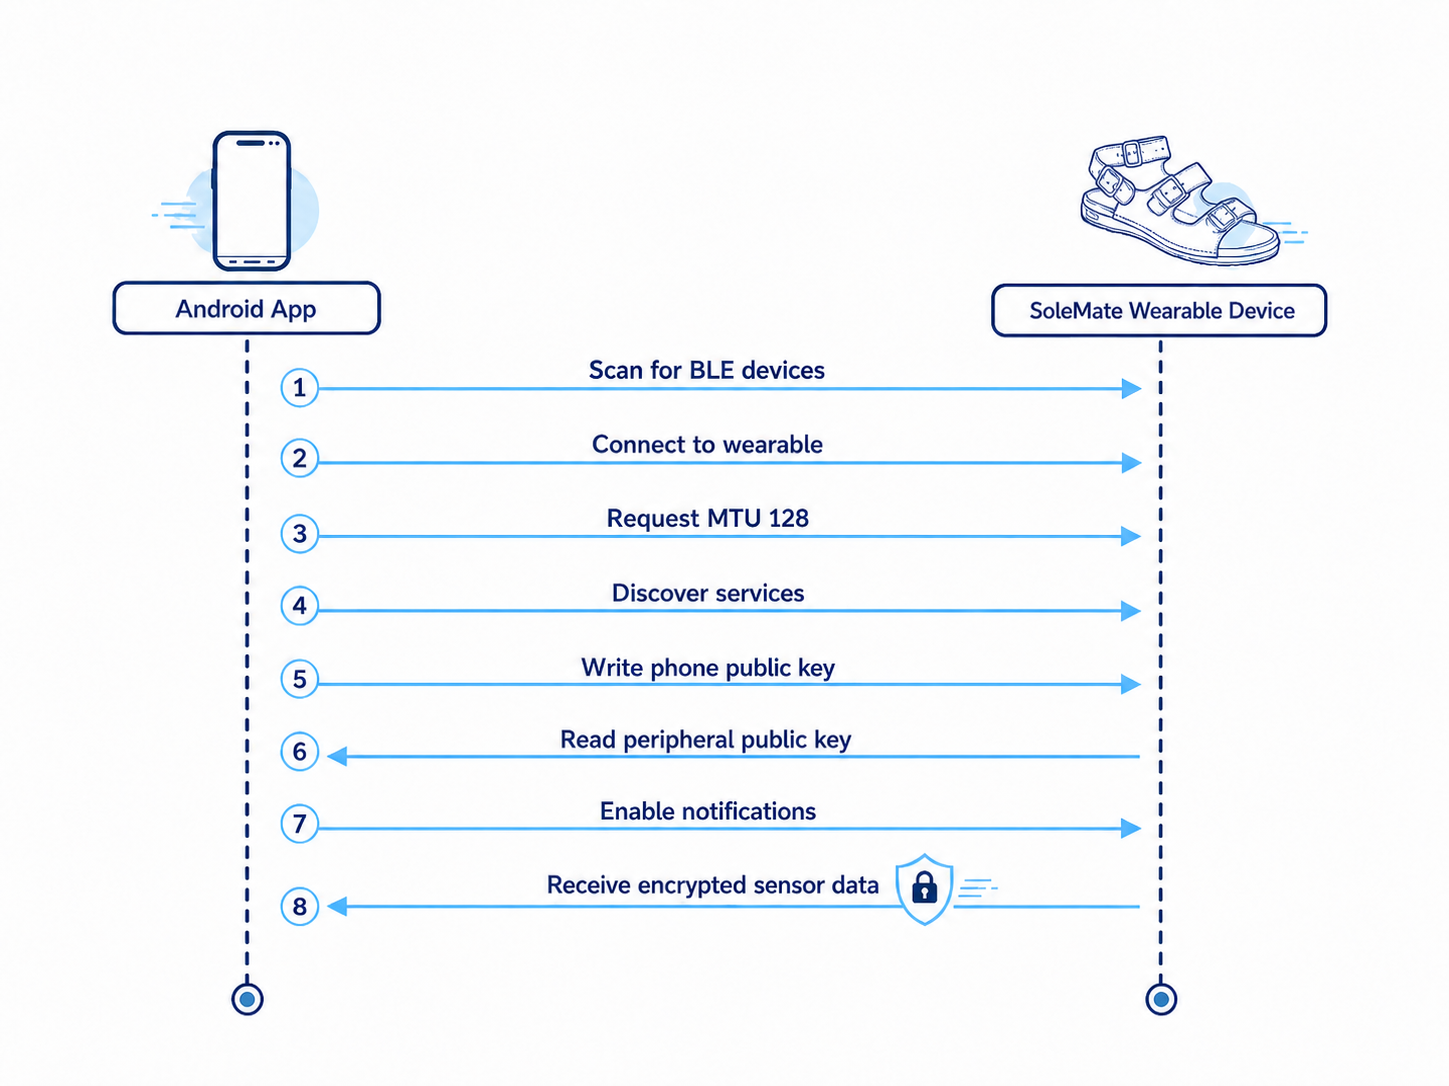
\includegraphics[width=0.95\textwidth]{FYP_Template_Spring/Figures/ble_seq.png}
  \caption{BLE connection and key-exchange sequence between Android and the wearable device.}
  \label{fig:ble_seq}
\end{figure}

% ------------------------------------------------------------
\section{Security Implementation}
\label{sec:security}
% ------------------------------------------------------------

\subsection{ECDH Key Exchange}
\label{subsec:sec_ecdh}

\noindent To avoid hard-coded shared secrets, SoleMate implements an Elliptic-Curve Diffie–Hellman (ECDH) handshake at the start of every BLE session.  Both the Arduino and the Android application
generate \textit{ephemeral} key pairs on the \textbf{secp256r1} (P-256) curve.  Public keys are
exchanged via the dedicated Key Exchange GATT characteristics and the ECDH shared secret is
computed independently on each side. \\

\noindent On the Android side the key exchange is handled by the \texttt{KeyExchangeManager} class
(\texttt{KeyExchangeManager.kt}), using Java's standard \texttt{javax.crypto.KeyAgreement} API
with the \texttt{"ECDH"} algorithm.  The public key is serialised in uncompressed form:
\texttt{0x04 || X || Y} (65 bytes), where X and Y are the 32-byte big-endian coordinates of the
public point.  On the Arduino side, the \texttt{key\_exchange} module uses the \texttt{uECC}
(micro-ECC) library for constrained-device curve arithmetic. \\

\noindent The private key and \texttt{KeyAgreement} instance are zeroed immediately after the shared
secret is derived (\texttt{close()} in the \texttt{AutoCloseable} implementation), reducing the
amount of long-lived secret material kept in memory. This provides a prototype-level form of
session separation: a later compromise of one session key does not directly reveal the keys used in
previous sessions. Since the current key exchange is not authenticated by certificates or a pairing
code, a production medical version would still require an authenticated pairing mechanism to resist
active man-in-the-middle attacks. \\

\noindent Algorithm~\ref{alg:ecdh} formalises the key exchange procedure.

\begin{algorithm}[htbp]
\caption{Session Key Exchange (ECDH, secp256r1)}
\label{alg:ecdh}
\begin{algorithmic}[1]
  \STATE \textbf{Both sides independently:} generate ephemeral key pair
         $(d_\text{self}, Q_\text{self})$ on secp256r1
  \STATE \textbf{Android} writes $Q_\text{phone}$ (65 bytes) to the Phone Public Key characteristic
  \STATE \textbf{Arduino} callback \texttt{onPhoneKeyWritten()} fires; reads $Q_\text{phone}$
  \STATE \textbf{Arduino} computes $S = d_\text{device} \cdot Q_\text{phone}$ (ECDH)
  \STATE \textbf{Android} reads $Q_\text{device}$ from Peripheral Public Key characteristic
  \STATE \textbf{Android} computes $S = d_\text{phone} \cdot Q_\text{device}$ (same shared point)
  \STATE \textbf{Both sides} derive 7 data-type keys from $S$ (see Section~\ref{subsec:sec_kdf})
  \STATE \textbf{Both sides} wipe ephemeral private key material from memory
\end{algorithmic}
\end{algorithm}

\subsection{AES-128-CBC Encryption and Key Derivation}
\label{subsec:sec_kdf}

\noindent From the raw ECDH shared secret $S$, seven 128-bit AES keys are derived — one per data type —
using a simple key-derivation function (KDF) based on SHA-256:

\begin{equation}
  k_i = \text{SHA-256}(S \mathbin{\|} \text{purpose}_i)[0:16]
  \label{eq:kdf}
\end{equation}

\noindent where $\text{purpose}_i$ is an ASCII string that uniquely identifies each data channel
(e.g.\ \texttt{"HEART\_RATE"}, \texttt{"SPO2"}, \texttt{"FLEX"}).  Using independent keys per
channel reduces direct key reuse between data types, although it does not replace the need for a
full, reviewed medical-device security design. \\


\noindent In the current prototype, each key is paired with a \textit{static} per-type initialisation
vector (IV), defined identically in both the Arduino firmware (\texttt{encryption.cpp}) and the
Android \texttt{AESCrypto} object. This choice simplified packet parsing on the constrained BLE
payloads, but it is a limitation of the prototype because CBC mode is stronger when each message
uses a fresh unpredictable IV. A future version should transmit a per-packet random IV or migrate
to an authenticated-encryption mode such as AES-GCM or ChaCha20-Poly1305. Table~\ref{tab:aes_ivs}
enumerates the seven IV ranges. \\

\begin{table}[htbp]
  \centering
  \caption{AES-128-CBC key-derivation purposes and prototype static IV byte ranges.}
  \label{tab:aes_ivs}
  \begin{tabularx}{\textwidth}{l l X}
    \hline
    \textbf{Data type} & \textbf{KDF purpose string} & \textbf{IV bytes (16-byte range)} \\
    \hline
    Steps (IMU)    & \texttt{STEPS}     & \texttt{0x00\ldots0x0F} \\
    Motion (IMU)   & \texttt{MOTION}    & \texttt{0x10\ldots0x1F} \\
    Heart rate     & \texttt{HEART\_RATE} & \texttt{0x20\ldots0x2F} \\
    SpO\textsubscript{2} & \texttt{SPO2} & \texttt{0x30\ldots0x3F} \\
    Flex / Edema  & \texttt{FLEX}      & \texttt{0x40\ldots0x4F} \\
    Pressure matrix & \texttt{PRESSURE} & \texttt{0x50\ldots0x5F} \\
    PPG waveform   & \texttt{PPG\_WAVE} & \texttt{0x60\ldots0x6F} \\
    \hline
  \end{tabularx}
\end{table}

\noindent All ciphertext is produced and consumed using \texttt{AES/CBC/PKCS5Padding}.  A legacy fallback
path (\texttt{initWithLegacyKeys()}) is available for firmware builds that pre-date the key
exchange service; in that mode, fixed compiled-in keys are used and the system degrades gracefully
without crashing. \\


\subsection{User Authentication and App Lock}
\label{subsec:sec_auth}

\noindent At the application layer, user accounts are protected by a password registered during
on-boarding and stored in Android SharedPreferences. An optional \textit{app lock} feature,
implemented via the AndroidX Biometric library, requires fingerprint or face verification every
time the application returns from background.  The \texttt{BiometricAuthHelper} utility class
encapsulates the \texttt{BiometricPrompt} lifecycle so that any activity can trigger
re-authentication with a single call. \\

\section{Android Application}
\label{sec:android}


\subsection{Application Architecture}
\label{subsec:android_arch}

The Android application (\texttt{minSdk} 26, \texttt{targetSdk} 34) consists of 31 Kotlin source
files organised around a hub-and-spoke Activity model.  Navigation flows from
\texttt{WelcomeActivity} through \texttt{RegistrationActivity} and \texttt{LoginActivity} to a
persistent \texttt{ScanActivity} that establishes the BLE session.  Once connected, a
\texttt{MainActivity} navigation drawer provides access to the principal feature screens.
Figure~\ref{fig:activity_nav} illustrates the navigation graph.

\begin{figure}[htbp]
  \centering
  \fbox{%
    \begin{minipage}{0.85\textwidth}
      \vspace{5.5cm}
      \centering
      \textit{[INSERT FIGURE: Activity navigation diagram showing Welcome
               $\rightarrow$ Register / Login $\rightarrow$ Scan $\rightarrow$
               Main (drawer: Readings, Gait, Pressure, Analytics, Settings)]}
      \vspace{5.5cm}
    \end{minipage}}
  \caption{Android application activity navigation graph.}
  \label{fig:activity_nav}
\end{figure}

\subsection{BLE Session Management}
\label{subsec:android_ble}

BLE scanning and initial device selection are performed from \texttt{ScanActivity}.  After the
user selects a device, \texttt{MainActivity} owns the \texttt{BluetoothGatt} callback pipeline:
connect with \texttt{connectGatt(applicationContext, \ldots)} (application context avoids drops when
navigating to analytics screens), delayed service discovery, ECDH key exchange when the Key Exchange
Service is present, then CCCD-enabled notifications for the wearable characteristics.
\texttt{BleGattSession} is a small singleton holder that retains the active \texttt{BluetoothGatt}
reference across \texttt{Activity} transitions.  When the Key Exchange Service is detected,
\texttt{KeyExchangeManager} writes the phone public key, reads the peripheral public key, and
\texttt{AESCrypto.init(sharedSecret)} derives per-channel AES keys; if the service is absent,
\texttt{AESCrypto.initWithLegacyKeys()} enables backwards-compatible operation.

\subsection{Data Decryption Pipeline}
\label{subsec:android_decrypt}

BLE notifications arrive on a background GATT callback thread.  Each notification handler
extracts the first byte of the payload as the ciphertext length, passes the remaining bytes to
the appropriate \texttt{AESCrypto.decrypt*} method, and posts the resulting string to the main
thread via a \texttt{Handler}.  Sensor-specific parsers then convert the ASCII string to typed
values (e.g.\ \texttt{Int} for BPM, \texttt{Float} for SpO\textsubscript{2}).  Pressure
notifications follow a different path: the 24-byte packet is validated against the
\texttt{0xA5~0x5A} magic, the 16-byte ciphertext is decrypted to 12 plaintext bytes by
\texttt{decryptPressurePayload()}, and the 8 twelve-bit samples are unpacked and inserted into
the current frame buffer.

% ------------------------------------------------------------
\section{Data Visualisation}
\label{sec:viz}
% ------------------------------------------------------------

\subsection{Vital Signs Charts}
\label{subsec:viz_vitals}

\texttt{ReadingsActivity} renders two real-time line charts using the MPAndroidChart
library~\cite{mpandroidchart}, one for heart rate (BPM) and one for SpO\textsubscript{2} (\%).
Each chart maintains a 30-point rolling window, rendered with cubic Bézier interpolation.
Colour-coded horizontal bands indicate clinical status zones (Normal, Elevated, Critical) so that
at-a-glance assessment is possible without numerical reading.  Figure~\ref{fig:viz_vitals} shows
the live readings screen.

\begin{figure}[htbp]
  \centering
  \fbox{%
    \begin{minipage}{0.45\textwidth}
      \vspace{6cm}
      \centering
      \textit{[INSERT SCREENSHOT: Readings Activity showing heart-rate and SpO\textsubscript{2}
               charts with colour zones]}
      \vspace{6cm}
    \end{minipage}}
  \caption{Vital-signs screen showing real-time heart rate and SpO\textsubscript{2} charts.}
  \label{fig:viz_vitals}
\end{figure}

\subsection{Plantar Pressure Heatmap}
\label{subsec:viz_pressure}

\texttt{PressureMatrixActivity} renders the 768-cell pressure frame as a colour heatmap on a
custom \texttt{Canvas} view.  Each cell is upscaled by a factor of approximately 40 to fill the
display area.  Three display modes are available:

\begin{itemize}[itemsep=2pt]
  \item \textbf{PIX} (precise): raw, unsmoothed 12-bit values mapped directly to a colour gradient.
  \item \textbf{DYNAMIC}: nearest-neighbour interpolation with a configurable smoothing kernel.
  \item \textbf{FIXED}: values are normalised against a fixed maximum, enabling inter-session
        pressure comparisons.
\end{itemize}

\noindent A calibration routine averages 100 baseline frames to subtract the device's own resting
impedance, so only genuine plantar load is displayed.  Three sub-views — \texttt{PlantarFootAnalyticsActivity}, \texttt{BigToeAnalyticsActivity}, and \texttt{AnkleCuffAnalyticsActivity} — provide
focused analytics for specific anatomical zones.  Figure~\ref{fig:viz_heatmap} shows the heatmap
and a zone analytics screen.

\begin{figure}[htbp]
  \centering
  \subfigure[Full plantar heatmap]{\fbox{%
    \begin{minipage}{0.42\textwidth}
      \vspace{6cm}
      \centering
      \textit{[INSERT SCREENSHOT: Pressure matrix heatmap in DYNAMIC mode]}
      \vspace{6cm}
    \end{minipage}}}
  \hfill
  \subfigure[Zone analytics view]{\fbox{%
    \begin{minipage}{0.42\textwidth}
      \vspace{6cm}
      \centering
      \textit{[INSERT SCREENSHOT: Big Toe / Plantar zone analytics screen]}
      \vspace{6cm}
    \end{minipage}}}
  \caption{Plantar pressure visualisation: full heatmap (left) and zone-based analytics (right).}
  \label{fig:viz_heatmap}
\end{figure}

\subsection{Gait and Edema Display}
\label{subsec:viz_gait}

\texttt{GaitAnalysisActivity} presents six real-time IMU traces ($a_x, a_y, a_z$;
$\omega_x, \omega_y, \omega_z$) alongside a colour-gradient bar that transitions from green
(no edema) through yellow and orange to red (severe edema) in proportion to the sensor
deviation reported by the firmware.  The numeric edema deviation and textual severity label are
displayed adjacent to the gradient bar for clinical clarity.


\section{Blood Pressure Estimation Pipeline}
\label{sec:bpml}

% ------------------------------------------------------------
\subsection{Dataset}
\label{subsubsec:bp_dataset}
% ------------------------------------------------------------

\noindent The model was trained on the \textbf{MIMIC~BP} dataset, a curated derivative of the MIMIC~III
waveform archive assembled specifically for cuffless blood pressure estimation research.
MIMIC~BP was preferred over the broader MIMIC~III waveform archive because its curation pipeline
enforces stricter arterial blood pressure (ABP) alignment and removes segments containing
flat-line artefacts or missing annotations, yielding higher label fidelity for supervised
regression. \\

\noindent Data were divided at the \emph{subject} level to prevent any information leakage between splits,
yielding 191{,}880 training segments, 41{,}220 validation segments, and 41{,}220 test segments.
Each segment corresponds to a 5-second window (625 samples at 125\,Hz), consistent with the
on-device input format described below.
Labels were kept in raw mmHg throughout; no label normalisation was applied.


% ------------------------------------------------------------
\subsection{Signal Preprocessing}
\label{subsubsec:bp_preproc}
% ------------------------------------------------------------

\noindent Blood pressure cannot be measured directly from a PPG waveform without reference cuffs; instead,
SoleMate uses a trained neural network to estimate systolic (SBP) and diastolic (DBP) blood
pressure from morphological and spectral features of the PPG signal. \\

\noindent The \texttt{BpModelRunner} class (\texttt{BpModelRunner.kt}) accepts a 625-sample integer array
corresponding to a 5-second PPG window sampled at 125\,Hz.
The preprocessing pipeline is summarised in Algorithm~\ref{alg:bp_preproc}.

\begin{algorithm}[htbp]
\caption{PPG Signal Preprocessing for BP Estimation}
\label{alg:bp_preproc}
\begin{algorithmic}[1]
  \REQUIRE Raw PPG window $\mathbf{x}_0 \in \mathbb{Z}^{625}$
  \STATE Convert to float: $\mathbf{x}_0 \leftarrow \text{float}(\mathbf{x}_0)$
  \STATE First derivative: $x_1[i] = x_0[i] - x_0[i-1],\; x_1[0] = 0$
  \STATE Second derivative: $x_2[i] = x_1[i] - x_1[i-1]$
  \FOR{each channel $c \in \{0, 1, 2\}$}
    \STATE Z-normalise: $x_c \leftarrow (x_c - \mu_c)\,/\,\sigma_c$
    \STATE Reflect-pad by $N_\text{FFT}/2 = 64$ samples on both ends
    \STATE Compute STFT with $N_\text{FFT}=128$, hop=32, rectangular window
    \STATE Retain one-sided spectrum: $F = N_\text{FFT}/2 + 1 = 65$ bins
    \STATE Apply log-magnitude: $\text{spec}_c[t,k] = \ln(1 + |\text{STFT}[t,k]|)$
  \ENDFOR
  \ENSURE Tensors: $\mathbf{x}_{0,1,2} \in \mathbb{R}^{1 \times 1 \times 625}$;
          $\text{spec}_{0,1,2} \in \mathbb{R}^{1 \times T \times 65}$
\end{algorithmic}
\end{algorithm}


% ------------------------------------------------------------
\subsection{Model Architecture}
\label{subsubsec:bp_arch}
% ------------------------------------------------------------

\noindent The blood-pressure model, \textbf{BPEstimationModel}, is a re-implementation of the
SpectroTemporalNet architecture seen in Figure~\ref{fig:bp_pipeline} proposed by Slap\-ni\v{c}ar et al.\ \cite{Slapnicar2019}.
It processes all three input channels in parallel through two complementary branches — a temporal
residual branch and a spectro-temporal branch — before merging them into a single regression
head that outputs SBP and DBP directly in mmHg.


\begin{figure}[H]
  \centering
  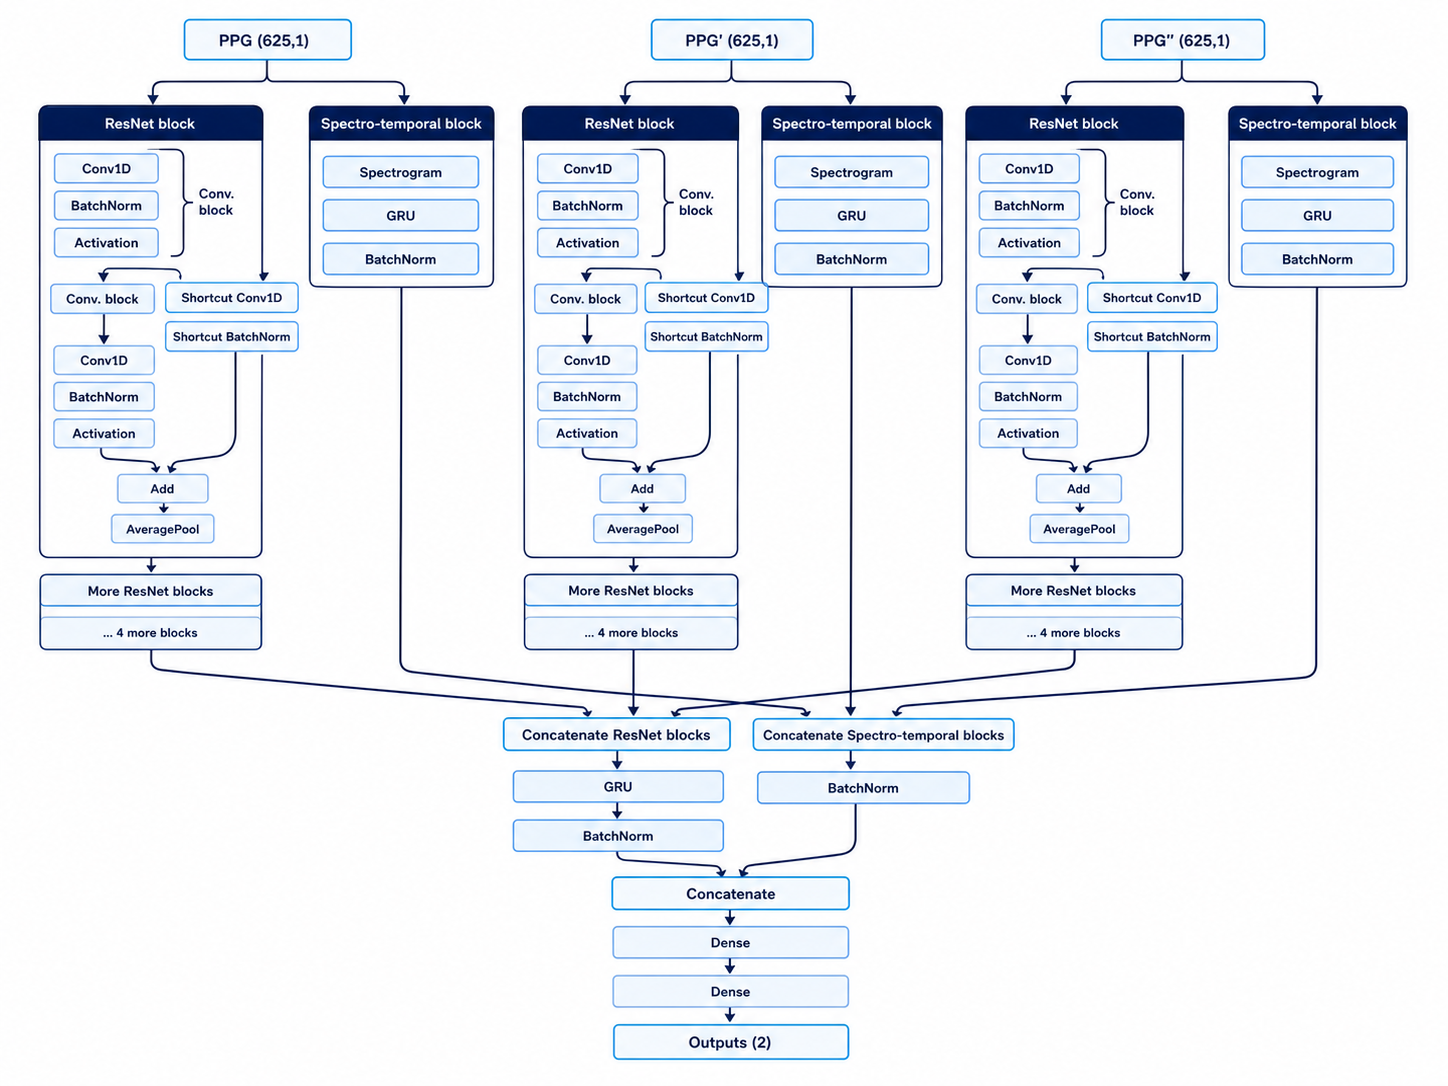
\includegraphics[width=\linewidth]{FYP_Template_Spring/Figures/bp_architecture.png}
  \caption{Blood-pressure estimation pipeline from raw PPG waveform to displayed prediction.}
  \label{fig:bp_pipeline}
\end{figure}

\paragraph{Temporal Residual Branch.}
Each input channel $\mathbf{x}_i \in \mathbb{R}^{1 \times 625}$ is processed by a dedicated
\textbf{ResNet branch} consisting of a stem convolution followed by five stacked residual blocks.
The structure is given in Table~\ref{tab:resnet_blocks}.
Each residual block applies two Conv1D--BatchNorm--ReLU paths whose outputs are summed with a
shortcut $1{\times}1$ convolution (applied only when channel dimensions change):
\[
  \mathbf{h} = \mathrm{ReLU}\!\bigl(\mathrm{BN}(\mathrm{Conv}(\mathbf{x}))
               + \mathrm{BN}(\mathrm{Conv}_{1\times1}(\mathbf{x}))\bigr).
\]
An \texttt{AdaptiveAvgPool1d(1)} at the end of the branch reduces the temporal dimension to a
single 128-dimensional feature vector.

\begin{table}[htbp]
  \centering
  \caption{Temporal residual branch configuration (per input channel).
           Stride\,$>$\,1 in blocks 3 and 5 performs spatial downsampling
           before the final global average pooling.}
  \label{tab:resnet_blocks}
  \small
  \begin{tabular}{lcccc}
    \toprule
    \textbf{Layer} & \textbf{In ch.} & \textbf{Out ch.} & \textbf{Kernel} & \textbf{Stride} \\
    \midrule
    Stem Conv + BN + ReLU & 1  & 32  & 3 & 1 \\
    Residual Block 1      & 32 & 32  & 3 & 1 \\
    Residual Block 2      & 32 & 32  & 3 & 1 \\
    Residual Block 3      & 32 & 64  & 3 & 2 \\
    Residual Block 4      & 64 & 64  & 3 & 1 \\
    Residual Block 5      & 64 & 128 & 3 & 2 \\
    AdaptiveAvgPool1d(1)  & -- & 128 & -- & -- \\
    \bottomrule
  \end{tabular}
\end{table}

\paragraph{Spectro-Temporal Branch.}
In parallel, each channel is passed through a \textbf{spectro-temporal branch}: a Short-Time
Fourier Transform ($N_\text{FFT}=128$, hop=32, rectangular window) produces a log-magnitude
spectrogram of shape $(T,\,65)$.
A unidirectional GRU (hidden size 64) processes the spectrogram frame by frame, and its final
hidden state yields a 64-dimensional spectral feature vector, followed by a BatchNorm layer.

\paragraph{Fusion and Regression Head.}
The three 128-dimensional residual features are stacked as a sequence $(B,\,3,\,128)$ and
processed by a \textbf{fusion GRU} (hidden size 128); its final hidden state is
batch-normalised to give a single 128-dimensional summary.
The three 64-dimensional spectral features are concatenated and batch-normalised to give a
192-dimensional spectral summary.
Both are concatenated to form a 320-dimensional fused representation, decoded by a two-layer
regression head:
\[
  \hat{\mathbf{y}} =
    \mathrm{Linear}_{64\to2}\!\bigl(
      \mathrm{Dropout}_{0.3}\!\bigl(
        \mathrm{ReLU}\!\bigl(
          \mathrm{Linear}_{128\to64}(
            \mathrm{Dropout}_{0.5}(\cdot)
          )
        \bigr)
      \bigr)
    \bigr),
\]
where $\hat{\mathbf{y}} \in \mathbb{R}^2$ contains the predicted SBP and DBP in mmHg.


% ------------------------------------------------------------
\subsection{Training Methodology}
\label{subsubsec:bp_training}
% ------------------------------------------------------------

\noindent Training proceeded in three successive phases, each motivated by an observed limitation of
the previous phase.
All phases shared a common base configuration: L1 (MAE) loss, a
\texttt{ReduceLROnPlateau} scheduler (reduction factor 0.5, LR-plateau patience 5 epochs,
minimum LR $10^{-7}$), gradient clipping at norm~1.0, early-stopping patience of 15~epochs,
and a fixed random seed of 42.

\paragraph{Phase 1 — Initial Training with RMSprop.}
The model was first trained using the hyperparameters reported in the original
paper~\cite{Slapnicar2019}: RMSprop with learning rate $10^{-4}$, $\alpha{=}0.99$,
momentum~0, weight decay $10^{-4}$, and batch size 256.
Inspection of the resulting training curves revealed that both training and validation MAE
were still trending downward at the early-stopping point, indicating that convergence had
not been reached and motivating a change of optimiser.

\paragraph{Phase 2 — Optimiser Switch to Adam.}
The optimiser was changed to \textbf{Adam} ($\beta_1{=}0.9$, $\beta_2{=}0.999$), with all
other settings held constant.
Adam's per-parameter adaptive learning rates produced faster convergence and a lower
validation loss, confirming a more favourable optimisation trajectory for this architecture
and motivating a systematic search of the wider hyperparameter space.

\paragraph{Phase 3 — Hyperparameter Grid Search.}
A systematic grid search was conducted over the following space:
\begin{itemize}
  \item \textbf{Optimiser}: Adam, RMSprop
  \item \textbf{Learning rate}: $\{10^{-4},\ 3{\times}10^{-4},\ 10^{-3}\}$
  \item \textbf{Batch size}: $\{128,\ 256\}$
  \item \textbf{Weight decay}: $\{10^{-4},\ 10^{-3}\}$
\end{itemize}
This yielded 24 configurations, each trained independently to early stopping from a fresh
random initialisation.
The configuration achieving the lowest validation MAE was selected as the final deployed model.


% ------------------------------------------------------------
\subsection{On-Device Deployment}
\label{subsubsec:bp_inference}
% ------------------------------------------------------------

\noindent The trained model is exported to the ExecuTorch portable format and stored as
\texttt{bp\_model.pte} (2.9\,MB) in the application's assets folder.
At runtime, \texttt{BpModelRunner} (\texttt{BpModelRunner.kt}) loads the model lazily on
first inference by copying the asset to the app's private file directory and calling
\texttt{Module.load()}.
A double-checked locking pattern ensures the model is initialised only once even under
concurrent requests. \\

\noindent The model accepts six named input tensors — the three normalised waveform channels and their
corresponding log spectrograms — and returns a single output tensor of shape $(1,\,2)$ whose
two floats are the predicted SBP and DBP in mmHg.
The uncertainty associated with PPG-derived blood pressure estimation is communicated to the
user as a $\pm6$\,mmHg band around the SBP prediction and a $\pm4$\,mmHg band around the
DBP prediction. \\


% ------------------------------------------------------------
\section{Plantar Heatmap MS Ataxia Classification Pipeline}
\label{sec:ataxia_ml}
% ------------------------------------------------------------

This section describes the implementation of a binary MS versus non-MS classifier trained on static plantar-pressure heatmaps offline using PyTorch. The classifier shares the same visual modality as the pressure-matrix view in SoleMate, establishing a direct link between the mobile application and the underlying clinical model. All configuration decisions are managed through a single central file to ensure that experiments remain reproducible and directly comparable across runs.

% ------------------------------------------------------------
\subsection{Dataset and One-Foot Derivation}
\label{subsec:ataxia_dataset}
% ------------------------------------------------------------

The dataset comprises \textbf{226 bilateral} plantar-pressure acquisitions from \textbf{62 non-MS} and \textbf{43 MS} participants. Since each bilateral image captures both feet on a single canvas, each image was split along the vertical mid-line to produce two independent single-foot crops. Left-foot crops were mirrored horizontally so that all samples share a consistent anatomical orientation. This derivation doubles the effective dataset size to \textbf{452 single-foot samples}, which is significant given the limited availability of clinical MS gait data. Labels are binary throughout (MS vs.\ non-MS).

% ------------------------------------------------------------
\subsection{Preprocessing}
\label{subsec:ataxia_preproc}
% ------------------------------------------------------------

Preprocessing is applied on-the-fly at load time rather than baked into a static archive, allowing preprocessing configurations to be changed between experiments without regenerating data. Each stage is independently toggleable so that their individual contributions to model performance can be evaluated in isolation. The pipeline stages are applied in a fixed canonical order, as summarised in Algorithm~\ref{alg:ataxia_preproc} and Table~\ref{tab:ataxia_preproc_flags}, and illustrated in Figure~\ref{fig:preproc_pipeline}.

\begin{figure}[htbp]
  \centering
  \includegraphics[width=0.95\textwidth]{figures/preprocessing_pipeline}
  \caption{On-the-fly preprocessing pipeline. Each stage is independently toggleable, allowing its contribution to model performance to be evaluated in isolation. The minimal path bypasses all optional stages and applies only resizing and intensity scaling.}
  \label{fig:preproc_pipeline}
\end{figure}

\begin{algorithm}[htbp]
\caption{On-the-fly preprocessing dispatch}
\label{alg:ataxia_preproc}
\begin{algorithmic}[1]
  \REQUIRE Raster colour footprint image $I$
  \IF{full preprocessing chain enabled}
    \STATE Optionally remove UI overlays via HSV masking
    \STATE Optionally suppress speckle noise
    \STATE Optionally crop to foreground bounding box with padding
    \STATE Optionally zero pixels outside the footprint mask
    \STATE Optionally remap intensities to ink-on-paper appearance
    \STATE Resize to network input resolution
    \STATE Apply per-image or global intensity scaling
    \STATE Form greyscale ($C{=}1$) or RGB ($C{=}3$) tensor
  \ELSE
    \STATE Minimal path: greyscale, resize, scale to $[0,1]$
  \ENDIF
  \ENSURE Tensor $\mathbf{x} \in [0,1]^{C\times H\times W}$, label $y$
\end{algorithmic}
\end{algorithm}

\begin{table}[htbp]
  \centering
  \caption{Configurable preprocessing stages.}
  \label{tab:ataxia_preproc_flags}
  \small
  \begin{tabularx}{\textwidth}{l X}
    \toprule
    \textbf{Stage} & \textbf{Purpose} \\
    \midrule
    Overlay suppression    & Remove non-physiological annotations introduced during acquisition \\
    Speckle filter         & Suppress compression noise that could mislead learned features \\
    Foreground crop        & Normalise spatial scale and framing across participants \\
    Background suppression & Reduce variance from inactive image regions \\
    Intensity remapping    & Standardise appearance across different capture conditions \\
    Resize                 & Match network input geometry (128$\times$128 or 224$\times$224) \\
    Intensity normalisation & Compensate for inter-subject pressure amplitude variation \\
    Channel mode           & Support both greyscale CapsNets and RGB pretrained encoders \\
    \bottomrule
  \end{tabularx}
\end{table}

% ------------------------------------------------------------
\subsection{Data Augmentation}
\label{subsec:ataxia_augment}
% ------------------------------------------------------------

Given the small dataset size, augmentation is important for preventing overfitting. Stochastic transforms are applied during training only; validation and held-out samples are preprocessed without augmentation to ensure unbiased evaluation. The implemented families---rotations, translations, brightness and contrast jitter, horizontal flipping, random scaling, Gaussian noise, and elastic warping---reflect the natural variability expected across clinical gait acquisitions. Each family is governed by a global enable flag, a magnitude bound, and a per-sample application probability, allowing fine-grained control during hyperparameter search, as listed in Table~\ref{tab:ataxia_aug_space}.

\begin{table}[htbp]
  \centering
  \caption{Augmentation families and tuned quantities.}
  \label{tab:ataxia_aug_space}
  \small
  \begin{tabular}{ll}
    \toprule
    \textbf{Family} & \textbf{Tuned quantities} \\
    \midrule
    Rotation            & On/off, angular span, apply probability \\
    Translation         & On/off, maximum shift fraction, probability \\
    Brightness/contrast & On/off, amplitude, probability \\
    Horizontal flip     & On/off, probability \\
    Scaling             & On/off, $(s_{\min}, s_{\max})$, probability \\
    Gaussian noise      & On/off, $\sigma$, probability \\
    Elastic warp        & On/off, stiffness and blur scale, probability \\
    \bottomrule
  \end{tabular}
\end{table}

% ------------------------------------------------------------
\subsection{Data Partitioning}
\label{subsec:ataxia_splits}
% ------------------------------------------------------------

A stratified partitioning scheme is used to preserve the MS/non-MS class ratio across all subsets. A \textbf{15\,\% withheld pool} is reserved before cross-validation begins and kept fixed across all experiments, providing an uncontaminated final evaluation set. On the remaining data, \textbf{5-fold cross-validation} is used to obtain reliable performance estimates despite the limited dataset size, with the validation fraction per fold determined by:
\[
  \mathrm{val\_frac} = \frac{1 - \mathrm{holdout\_frac}}{K}.
\]

Where multiple crops originate from the same acquisition, grouped cross-validation is applied to ensure correlated samples are never split across folds, which would otherwise cause data leakage and inflate validation metrics. Class-frequency-aware weighted sampling is optionally applied during training to address the MS/non-MS class imbalance.

% ------------------------------------------------------------
\subsection{Model Architectures}
\label{subsec:ataxia_models}
% ------------------------------------------------------------

Three classifier architectures were implemented and evaluated, motivated by different trade-offs between inductive bias, data efficiency, and representational capacity. All three share the same data loading and preprocessing pipeline.

\subsubsection{End-to-End Capsule Network}
\label{subsubsec:arch_capsnet}

CapsNets were chosen as the primary architecture because their equivariant routing mechanism captures spatial pose relationships in the foot pressure distribution---properties that are poorly represented by standard pooling operations. The network consists of a five-stage convolutional backbone (32$\rightarrow$64$\rightarrow$128$\rightarrow$256$\rightarrow$256 channels) feeding into primary and digit capsules using Sabour-style dynamic routing over three iterations. Two digit capsules represent the MS and non-MS classes, with classification driven by capsule vector norms $\lVert \mathbf{v}_c \rVert$.

An optional reconstruction decoder is included to regularise training by encouraging capsule poses to encode spatially meaningful features rather than collapsing to discriminative shortcuts. The composite objective is:
\[
  \mathcal{L} =
    \mathcal{L}_{\mathrm{margin}}\!\bigl(\{\lVert \mathbf{v}_c\rVert\}_{c=1}^2,\,\mathbf{y}\bigr)
    + \lambda_{\mathrm{rec}} \cdot \mathrm{MSE}(\hat{\mathbf{x}},\,\mathbf{x}).
\]

\begin{figure}[htbp]
  \centering
  \includegraphics[width=0.88\textwidth]{figures/arch_capsnet}
  \caption{End-to-end CapsNet architecture. The convolutional backbone produces spatial feature maps that are reshaped into primary capsules. Dynamic routing propagates pose votes to two digit capsules (MS and non-MS), with an optional reconstruction decoder added as a regularisation branch.}
  \label{fig:arch_capsnet}
\end{figure}

\subsubsection{Hybrid Pretrained CNN with Capsule Head}
\label{subsubsec:arch_cnn_caps}

To explore whether richer visual features could benefit the capsule routing stage, a hybrid architecture was implemented that attaches a capsule head to an ImageNet-pretrained backbone (ResNet, DenseNet, or MobileNet). The backbone provides general-purpose visual features without requiring large amounts of domain-specific training data, while the capsule head retains the spatial reasoning properties described above. The backbone can optionally be frozen, which reduces the risk of overfitting on the small medical imaging dataset while still allowing the capsule parameters to be adapted to the task.

\begin{figure}[htbp]
  \centering
  \includegraphics[width=0.88\textwidth]{figures/arch_cnn_caps}
  \caption{Hybrid CNN+capsule architecture. A pretrained backbone extracts visual features which are projected into primary capsule slots and routed to digit capsules. The backbone trunk can optionally be frozen to reduce overfitting on the limited training set.}
  \label{fig:arch_cnn_caps}
\end{figure}

\subsubsection{Deep Embeddings with a Support-Vector Machine}
\label{subsubsec:arch_cnn_svm}

A CNN+SVM baseline was included to provide a point of comparison against a well-established non-end-to-end approach. Embeddings are extracted from the penultimate layer of a fixed VGG-19 network and used to train a kernel SVM. Because the CNN weights are never updated, this approach avoids overfitting during the classification stage entirely, making it a useful reference for gauging how much the learned capsule representations add over generic deep features.

\begin{figure}[htbp]
  \centering
  \includegraphics[width=0.85\textwidth]{figures/arch_cnn_svm}
  \caption{CNN+SVM baseline. A fixed VGG-19 backbone extracts a feature embedding from its penultimate layer, which is optionally $\ell_2$-normalised before being passed to a kernel SVM for binary classification.}
  \label{fig:arch_cnn_svm}
\end{figure}

% ------------------------------------------------------------
\subsection{Hyperparameter Optimisation}
\label{subsec:ataxia_optuna}
% ------------------------------------------------------------

The large number of interacting hyperparameters---spanning augmentation, routing stability, and learning-rate adaptation---made manual search impractical. Automated optimisation was therefore performed using \textbf{Optuna} with a \textbf{Tree-structured Parzen Estimator (TPE)} sampler, which builds a probabilistic model of the objective surface to direct trials toward promising regions rather than sampling blindly. A \textbf{median pruner} terminates unpromising trials early based on intermediate validation accuracy, reducing wasted computation on the limited GPU budget available. Table~\ref{tab:optuna_space_snapshot} summarises the categories explored.

\begin{table}[htbp]
  \centering
  \caption{Hyperparameter categories explored by Optuna (non-exhaustive).}
  \label{tab:optuna_space_snapshot}
  \small
  \begin{tabular}{ll}
    \toprule
    \textbf{Category} & \textbf{Representative quantities} \\
    \midrule
    Optimisation      & Learning rate, batch size $\in\{8,16,32\}$, Adam vs.\ AdamW, weight decay \\
    Stability         & Gradient clip norm, mixed precision, routing iteration count \\
    Margin loss       & $m^{+}$, $m^{-}$, $\lambda_{\mathrm{margin}}$ \\
    Reconstruction    & On/off, $\lambda_{\mathrm{rec}}$, routing-logit clamp \\
    Scheduler         & Plateau patience, decay factor, minimum learning rate \\
    Augmentation      & See Table~\ref{tab:ataxia_aug_space} \\
    Capsule geometry  & Primary capsule count and vector dimension \\
    Hybrid trunk      & Frozen vs.\ trainable backbone \\
    \bottomrule
  \end{tabular}
\end{table}

% ------------------------------------------------------------
\subsection{Training Procedure}
\label{subsec:ataxia_training}
% ------------------------------------------------------------

All models are trained using Adam or AdamW with a reduce-on-plateau learning-rate schedule, chosen for its robustness to the noisy validation curves typical of small medical datasets. Automatic mixed precision is used where numerically stable to reduce memory usage; capsule routing is kept in full precision when half-precision causes overflow. Global gradient norm clipping is applied throughout to prevent instability during the routing backward pass.

The best-performing checkpoint from each fold is retained, and the fold with the highest validation score is promoted as the final model for evaluation. Per-epoch loss and accuracy are recorded to structured JSON logs to support post-hoc analysis and reproducibility.